\documentclass[11pt]{article}

\usepackage{geometry}                % See geometry.pdf to learn the layout options. There are lots.
\geometry{letterpaper}                   % ... or a4paper or a5paper or ... 
%\geometry{landscape}                % Activate for for rotated page geometry
%\usepackage[parfill]{parskip}    % Activate to begin paragraphs with an empty line rather than an indent
\usepackage{graphicx}
\usepackage{xcolor}
\usepackage{amssymb}
\usepackage{epstopdf}
%\usepackage{enumitem}
\usepackage{ulem}
\DeclareGraphicsRule{.tif}{png}{.png}{`convert #1 `dirname #1`/`basename #1 .tif`.png}
\usepackage{caption}
\usepackage{subcaption}
\title{URM Hanger Installation}
\author{Ryan Bayes}
\date{\today; V2}


\begin{document}
\maketitle

\section{Introduction}
The calibration deployment system needed to be updated in a number of ways to deploy sources in the scintillator filled UI. The URMs were redesigned to be leak tight and made out of scintillator compatible materials. Consequently, the URMs heavier than in water phase. Furthermore, it is assumed that the UI can move by as much as 8 inches vertically and 2 inches laterally. Finally, the gate valves selected for scintillator phase cannot take the torsional  stress of cantilevering a URM from it. For these reasons a new URM lifting system was designed. This new lifting and support system holds all of the weight of the URM independent of the UI assuming that the source tube is a flexible bellows.

The initial structural engineer design report indicated that the DCR Ibeam webbing cannot take the torsional stress of supporting the entire URM from the bottom flange alone, motivating a solution which supported the rear of the URM from below using a scissor lift cart and reinforced the front hanger to support the rails over the UI. The reinforced hanger is designed to wrap around the I-beam to reduce the stress on the interior webbing. The new design forces the installation team to work above the UI inside the DCR while breaking the DCR seal. As such, special precautions must be taken to keep the area outside of the working space clean.

\section{Definitions and Terms}
\begin{itemize}
\item {\bf URM}; Umbilical Retrieval Mechanism - System equipped to raise and lower sources by simultaneously manipulating the available length of a rope and umbilical attached to a source. 
\item {\bf URM Front Hanger} - A device clamped to the DCR I-beam which supports the URM over the UI by way of turnbuckles at the front of the UI. Also has rollers mounted for the lifting straps that support the rails when they are not supported by the turnbuckles. See Fig.\ref{fig:FHAClamp}.
\item {\bf URM Rear Hanger} - A device clamped to the DCR I-beam that supports the rollers for the rear lifting straps. It is not intended to lift the URM but it does provide some lateral safety during the lifting procedure. 
\item {\bf Scissor Cart} - A cart designed to support the URM and lift it to operating height prior to use. 
\item {\bf Lifting winch} - A device meant to wind straps that support the rails when not supported by the turnbuckles
\item {\bf Scaffold} - A temporary structure over the UI to be constructed specifically for this job, providing a foot path at least 152 cm (60 inches) above the Deck. The scaffold will have guard rails to prevent falls from the structure allowing workers to operate without harnesses and lanyards.
\item {\bf AV}; Acrylic Vessel - The centre of the SNO+ detector containing the active scintillator volume
\item {\bf AV neck} - A 7 metre long cylinder that connects to the spheroidal main body of the AV. 
\item {\bf UI}; Universal interface - The cap on the top of the AV neck consisting of the lower UI through which tubes for recirculation and extracting samples from the AV are connected, and the upper UI through which ports for gas lines, level sensors and calibration equipment exist. 
\item {\bf DCR}; Deck clean room - a tent in the centre of the SNO+ deck to isolate activities about the UI that may introduce contamination into the experiment from the rest of the lab. Is equipped with multiple hepa filters to circulate and clean the air that passes into the facility. 
%\item {\bf Radon monitor} - A 3 m$^{3}$ vacuum vessel used to measure levels of radon daughters in the cover gas volume. It is connected to the UI cover gas through a 1" diameter bellows hose. 
%\item {\bf Side rope motor box} - One of four boxes cantilevered off of the UI. Used to adjust the tension on the ropes used to guide sources in a 2-dimensional plane in the UI (either XZ or YZ). Necessarily connected to the UI cover gas through a 1/2" tube containing the side rope. All four motor boxes are equipped with quick connects to facilitate a clean connection to the UI cover gas space.
%\item {\bf Side rope extension box} - One of four boxes used to align the side rope with a feed through to enter the UI. Connected to the siderope motor box via a 1/2" inch tube with VCR connections on both ends. Connected to the UI cover gas through the rope feedthrough. Two extension boxes are equipped with valves to allow for clean connections to the UI cover gas.  
\end{itemize}

\section{Pre-Requisites}
Installing the URM front hanger will physically alter the DCR envelope with the potential for affecting the cleanliness of the environment. Precautions will be taken to make this as simple and efficient as possible. All of the parts must be identified and close at hand prior to starting work. Knowing the working environment well prior to the installation is essential for all workers. Safety is a number one priority and precautions must be taken to ensure that the installation goes ahead with a minimum of risk to the workers involved. The environmental considerations and risk mitigations are described below.

\subsection{Personnel}
\begin{itemize}
\item Task Lead: Ryan Bayes
\item Second: Matt Depatie
\item Further assistance: Parmesh Ravi, Stefan Kaluzienski
\item Scaffolding Assembly: Ben Zalan
\end{itemize}

\subsection{Parts and Equipment List}
\begin{itemize}
\item UI drop sheet
\item Temporary dust tent
\item Assembled scaffold over UI (Suggested height; 60 inches above DCR deck)
\item Knee pads for each of the workers involved (at least 2 pairs)
\item Heat resistant gloves for the workers (at least 2 pairs)
\item URM Front hanger consisting of
	\begin{itemize}
	\item Top plate (C-channel with 8 bolt holes for beam clamps on the wide surface and 3 bolt holes on the narrow surfaces)
	\item 2 side plates (L-bracket with 3 bolt holes near the end of the wide surface and 4 bolt holes on the narrow surface)
	\item Horizontal struts with bar installed using supports
	\item 16 beam clamp washers
	\item 16 stainless steel 5/8"-11 thread bolts, nuts and washers (8 partial washers to account for welds inside horizontal C-beam.
	\item 6 stainless steel 1/2" - 13 thread bolts  with 6 nuts and 12 washers
	\item 8 stainless steel 1/2" - 13 thread bolts  with 8 nuts and 16 washers
	\item 4 turnbuckles (install south pair only)
	\end{itemize}
\item URM Rear Hanger
	\begin{itemize}
	\item Horizontal struts with roller bar
	\item 8 beam clamp washers
	\item 8 zinc plated 5/8"-11 thread bolts, 
	\item 8 nuts and washers
	\end{itemize} 
\item new URM Winch 
	\begin{itemize}
	\item Winch assembly
	\item Old bolts to secure the winch to structural steel
	\end{itemize}
\item Wrenches
	\begin{itemize}
	\item 15/16" to secure the beam clamps
	\item 3/4" to secure the side plates
	\end{itemize}
\item Hex Socket wrenches
	\begin{itemize}
	\item 15/16" to secure the beam clamps
	\item 3/4" to secure the side plates
	\end{itemize}
\item Metal shears (sufficient to cut 1/8" aluminum)
\item 40"$\times$11" piece of tarp
\item Hot glue
\item Hot glue gun
\item cordless drill (with charged battery pack)
\item 3/8" hex drill socket
\end{itemize}

\begin{figure}[htbp]
\begin{center}
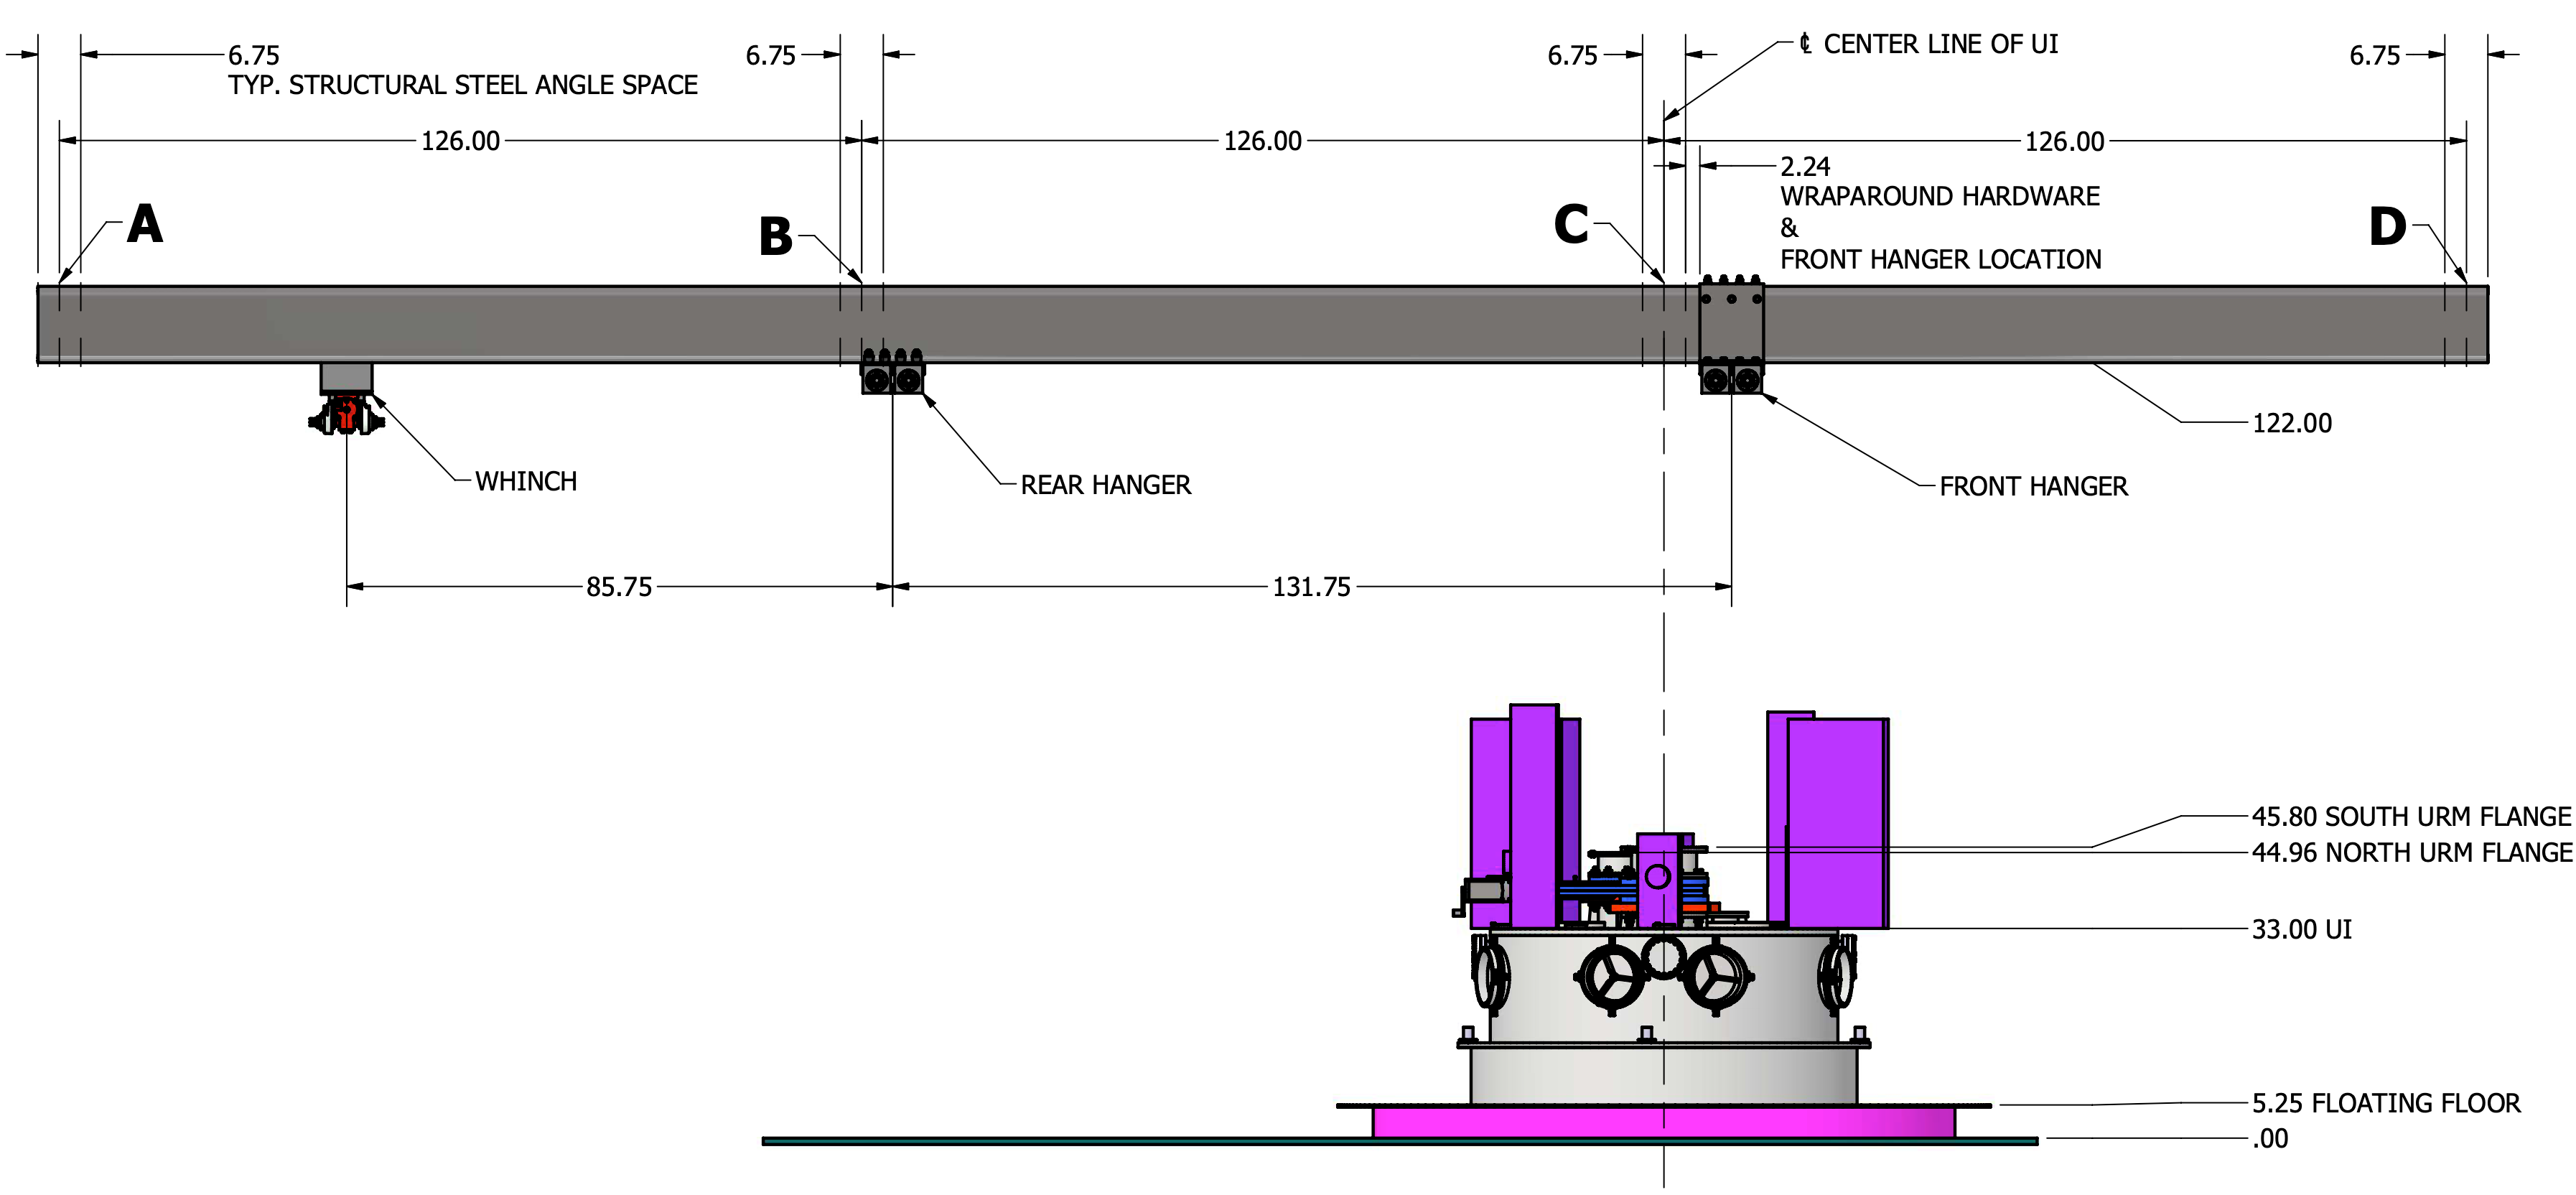
\includegraphics[width=\textwidth]{HangerBeamDimensions.png}
\caption{Location of the hangers and winch on the beam relative structural steel indicated (UI viewed from the South).}
\label{fig:hangerloc}
\end{center}
\end{figure}

\begin{figure}[htbp]
\begin{center}
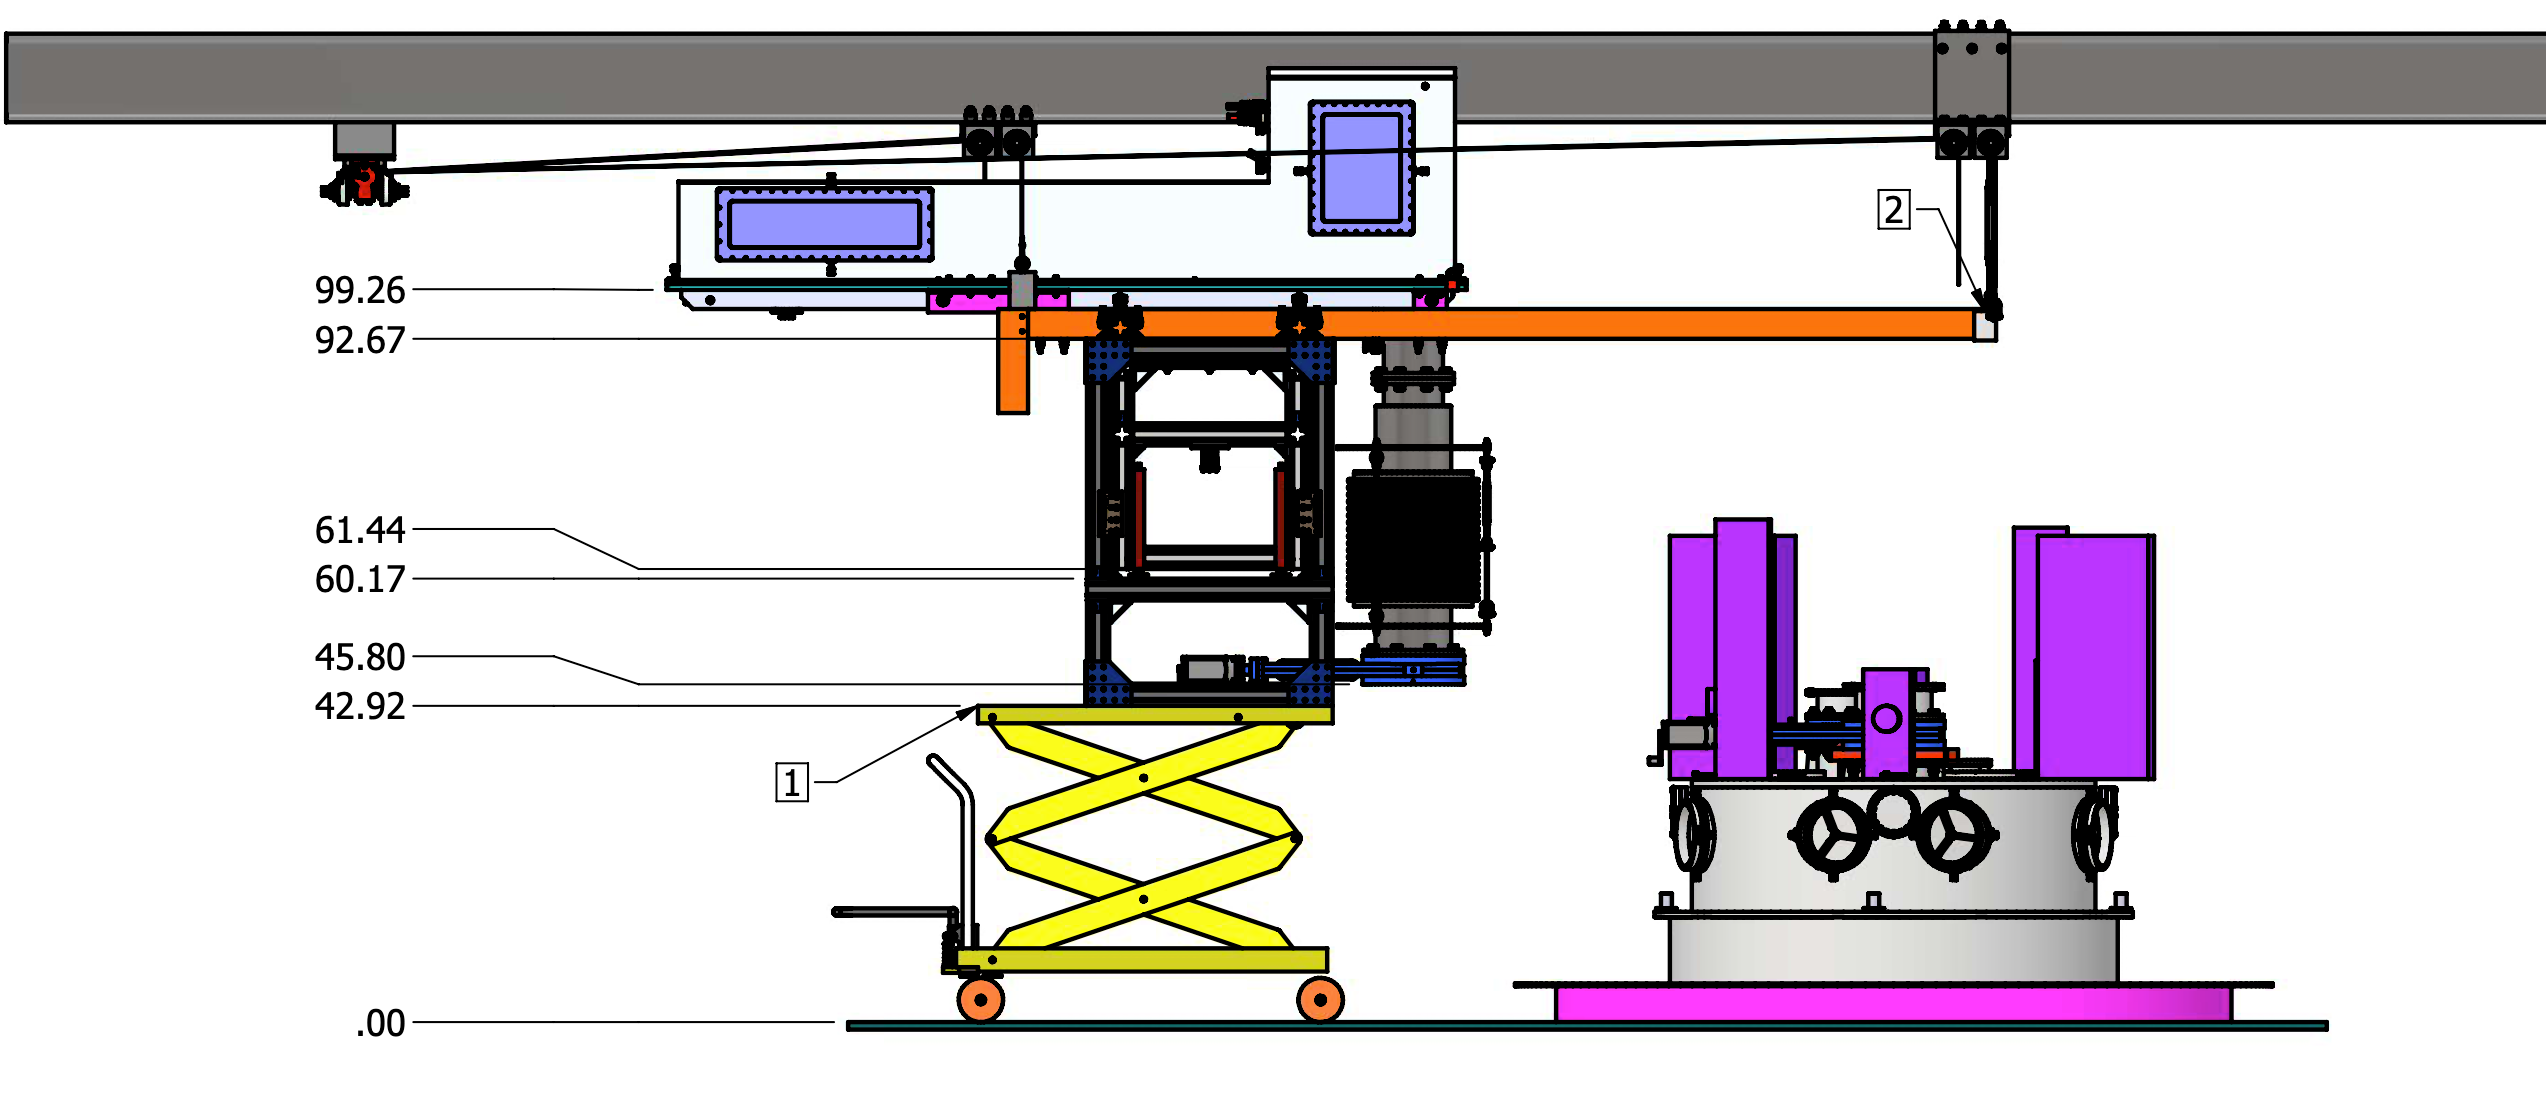
\includegraphics[width=\textwidth]{AssembledMechanismWithURM.png}
\caption{Assembled URM support system with the vertical dimensions of the various components.}
\label{default}
\end{center}
\end{figure}



\subsection{Environmental considerations}
When designing the new URM front hanger, the primary consideration was structural strength given the load at the required toque. No consideration was made to the integrity of the clean tent. The tent will need to be altered to renew the seal on the tent after the hanger installation. As a piece of c-channel is to be used to enclose the I-beam from the top, a breach must be made in the DCR tent. The tent will have to be resealed against the I-beam. At present the a tarp bag is suspended about the I-beam using a pair of 1"$\times$1" L-brackets clamped to the edge of the top face of the beam. These angle brackets will need to be removed and replaced with a series of shorter L brackets. The suggested approach is to replace the Then the bag can be rehung and closed. 

The DCR tent itself is sealed against the I-beam using double sided tape. Gaining access to the beam is as simple as pealing the tarp from the tape in a long enough section to complete the installation with a few small cuts to allow the remaining sections to be left in tact. A method to reseal the tarp after installation of the clamp would be to thread a piece of tarp underneath the vertical plates of the hanger so that the lower strut clamp grabs on to the new tarp and the bag. The new piece of tarp could be resealed against the I-beam and then threaded around the top bracket of the hanger so that sealing the tarp against itself forms a pocket for the top flange. If the piece of tarp cut from the DCR roof is threaded between the two vertical plates prior to bolting them together, the new seal can be produced while providing tension to the DCR roof.

The location of the hanger to be installed is offset 10cm from the centre-line of the acrylic vessel. This location is covered on the outside of the DCR tent with a plate that supported the feedthroughs for the SNO side rope motor boxes. This plate will need to be navigated during the installation of the plate to go over the I-beam which is considered feasible as the planned c-channel to be used for the upper part of the hanger clamp will be 3.45" high and the plate is supported 4" from the I-beam. However, the plate may help while the tent is breached as it will also serve as a partial dust shield from the deck environment.

The hanger installation will involve exposing the I-beam so a drop cloth must be placed over the UI to keep potential flakes from the I-beam or material from the scaffolding assembly from falling on the UI. The proposed drop cloth will be composed of polysheet plastic and should cover the UI out to the edge of the sliding floor. A partial dust tent should be maintained around the scaffolding during the installation itself to control the spread of dust to the immediate vicinity. 


\begin{figure}[htbp]
\begin{center}
	\begin{subfigure}{0.45\textwidth}
	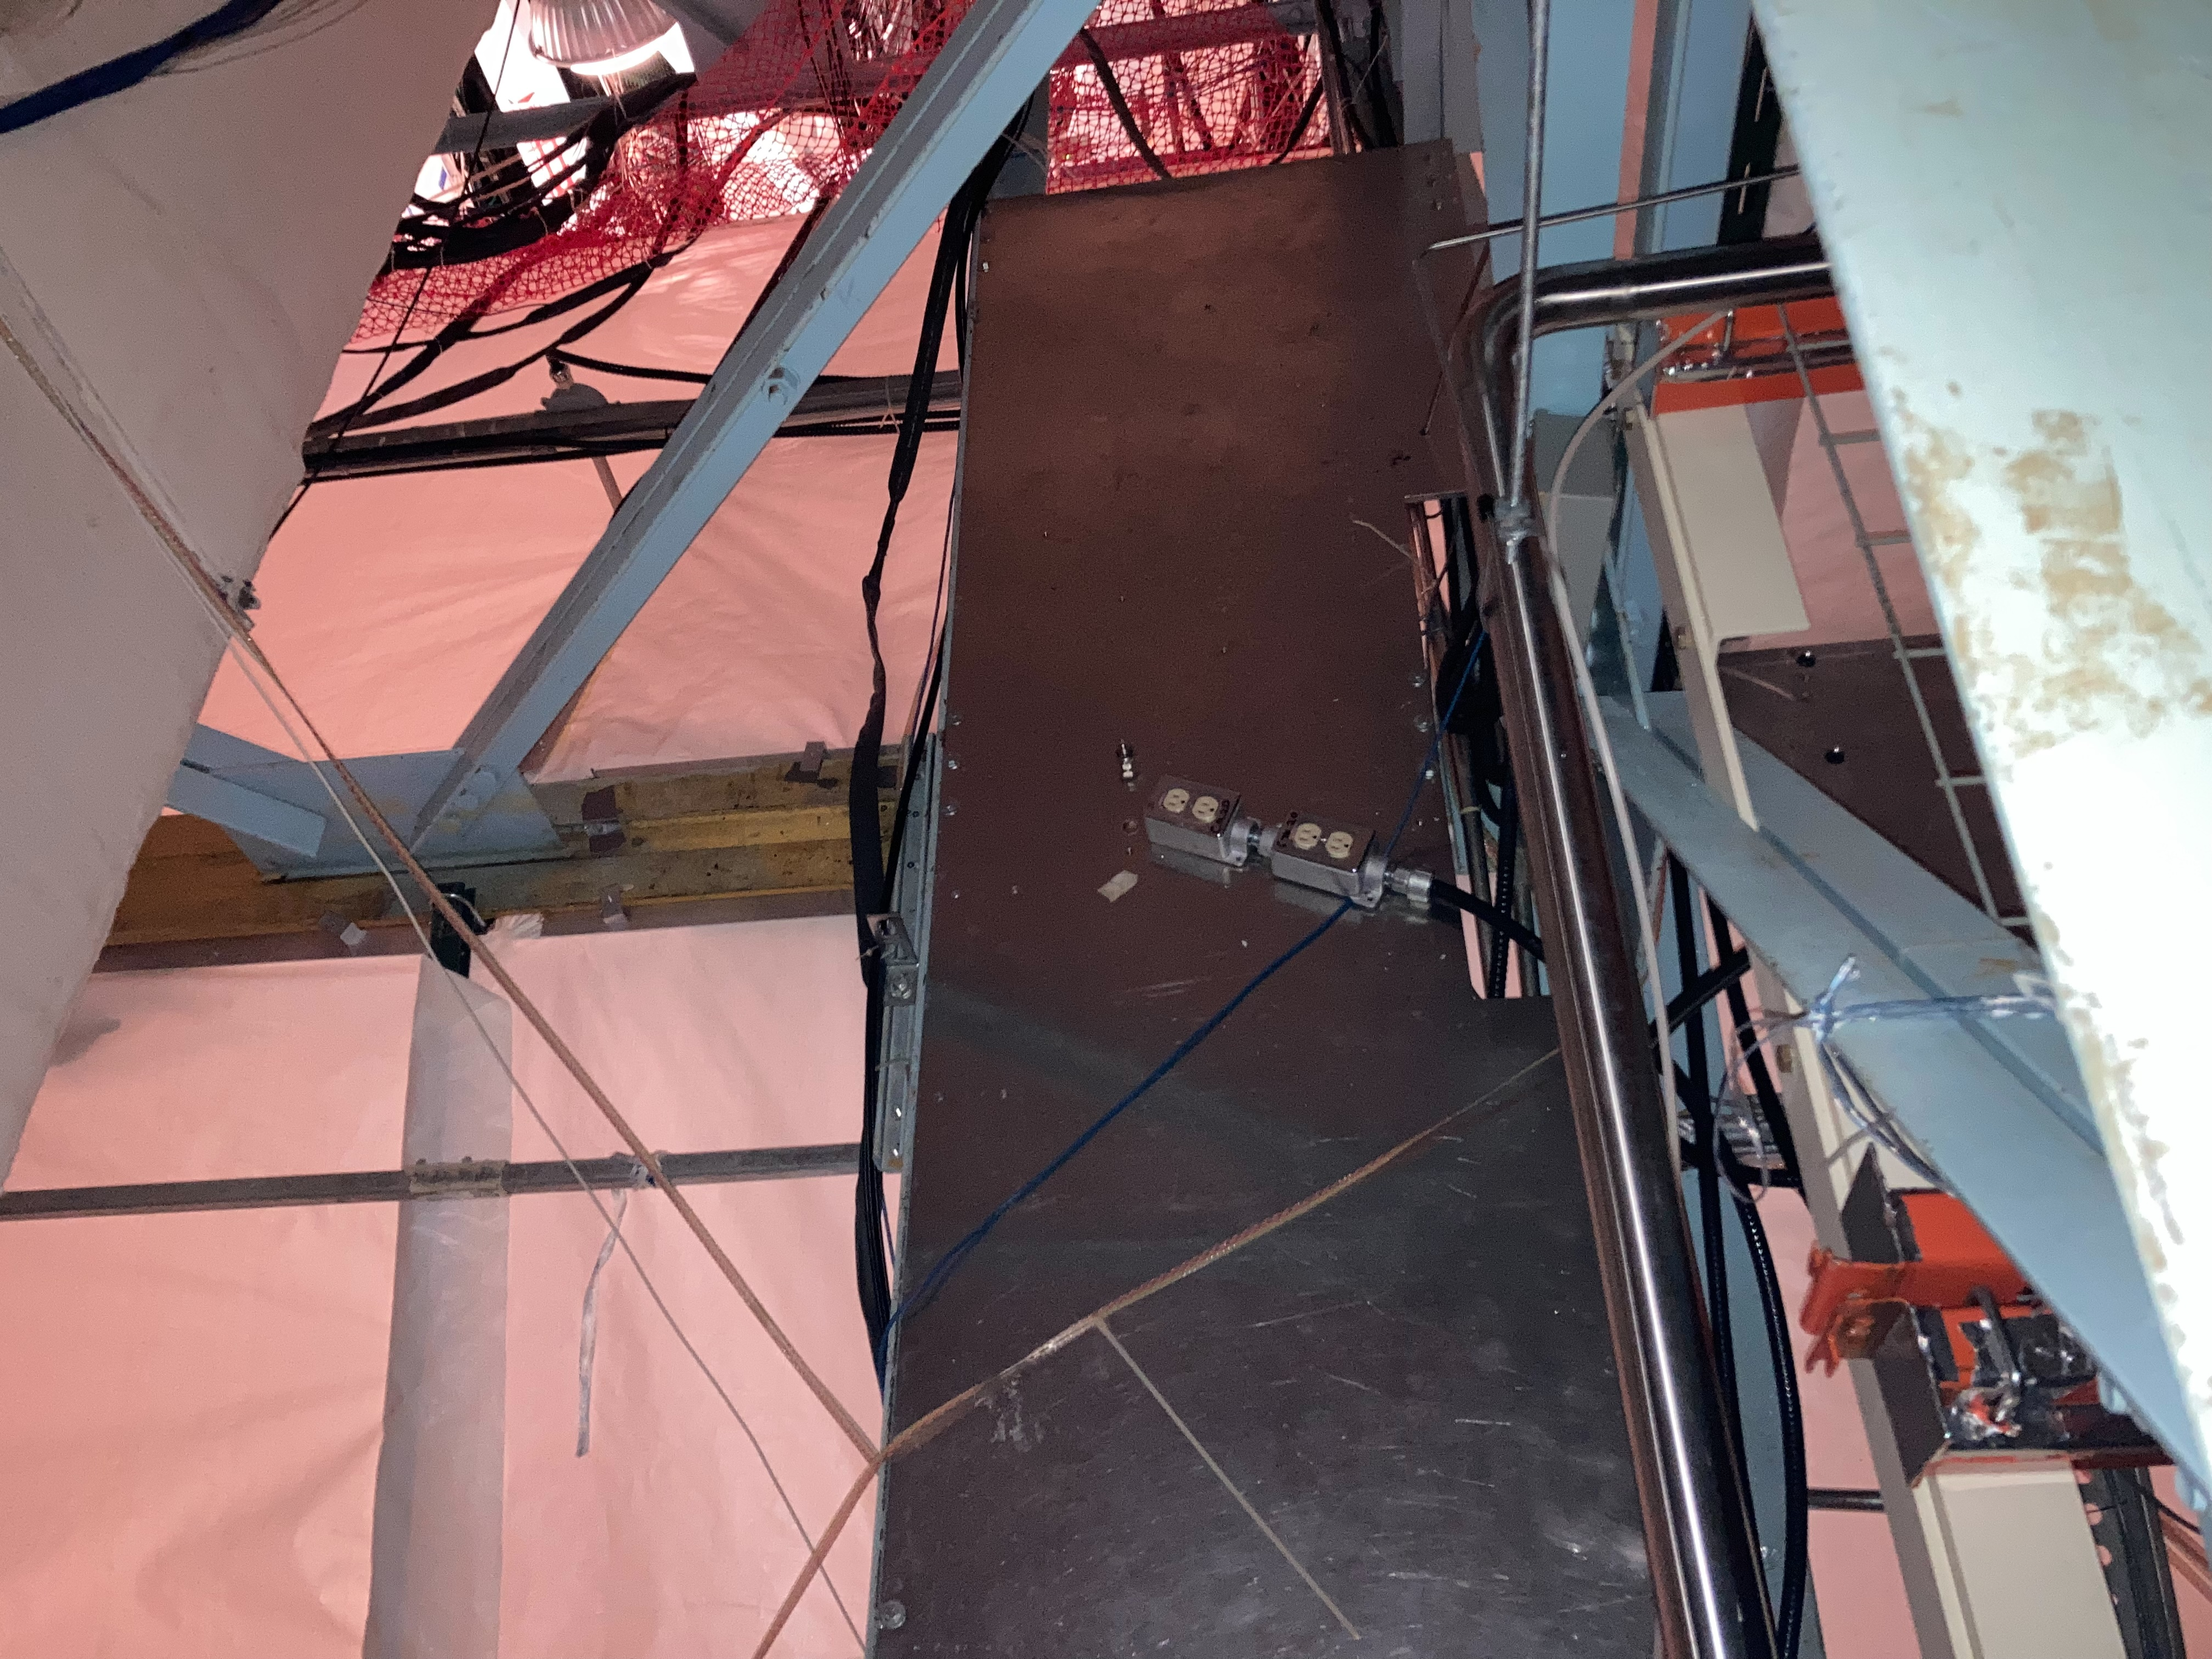
\includegraphics[width=\textwidth]{TopOfDCR}
	\caption{View of the top of the DCR from the existing covergas scaffolding.}
	\label{fig:topofDCR}
	\end{subfigure}
	\begin{subfigure}{0.45\textwidth}
	\includegraphics[width=\textwidth]{CoveredIbeamNorth}
	\caption{View of the North face of the covered I-beam}
	\label{fig:cvIbeamN}
	\end{subfigure}
	\begin{subfigure}{0.45\textwidth}
	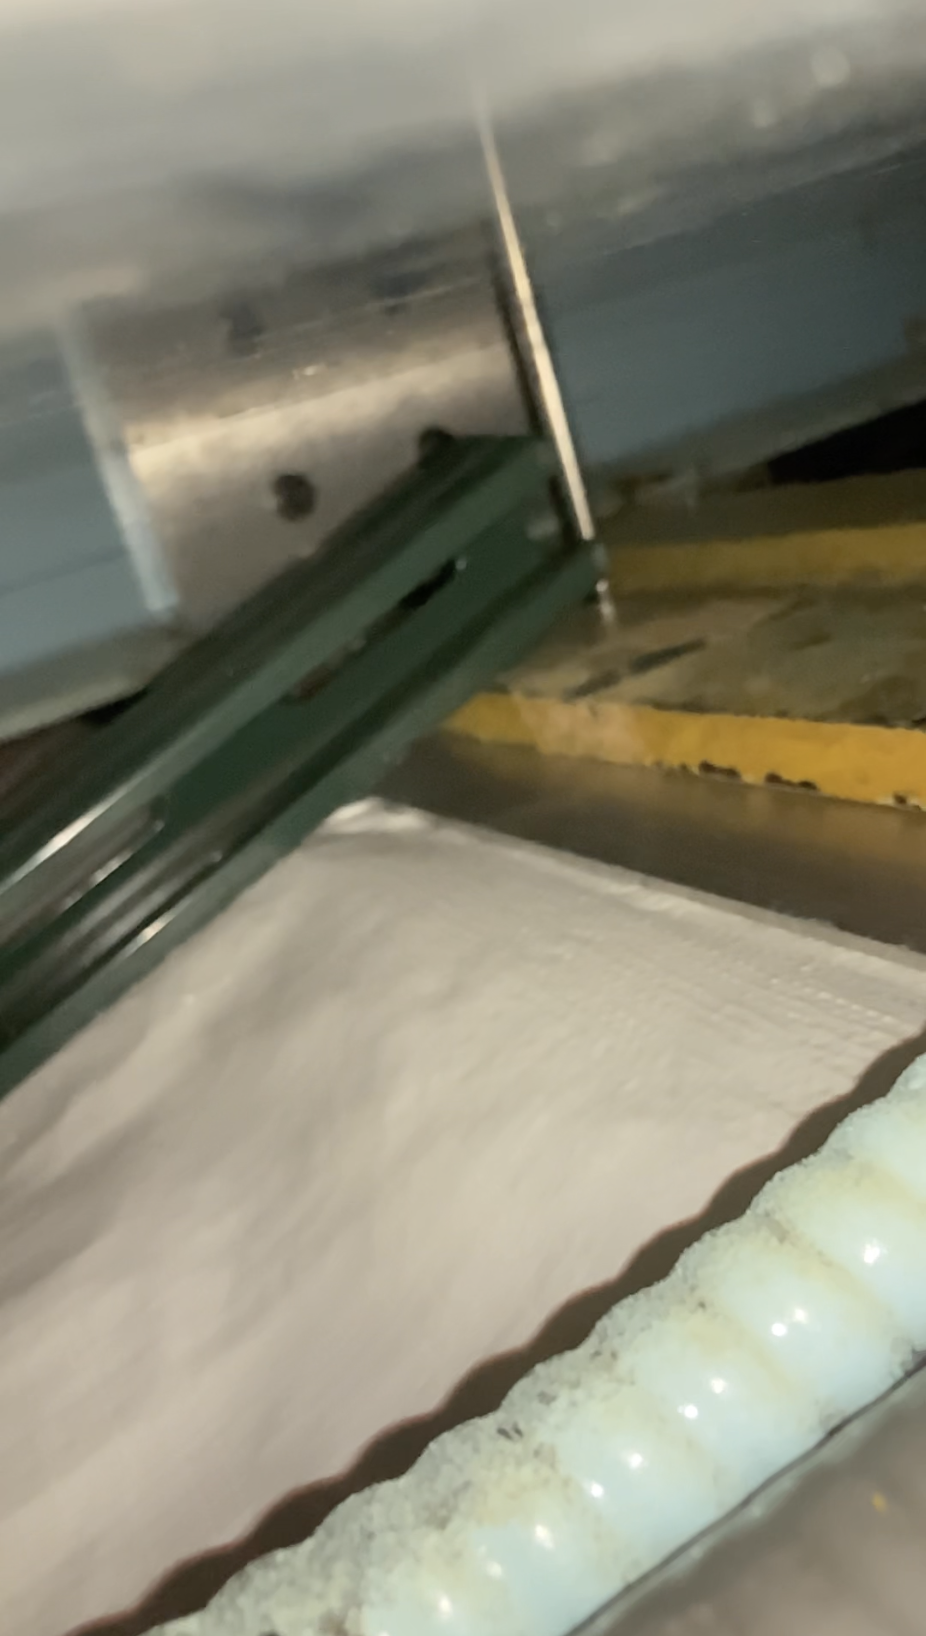
\includegraphics[width=\textwidth]{UnderPlate}
	\caption{View of the underside of the SNO siderope plate.}
	\label{fig:belowplate}
	\end{subfigure}
	\begin{subfigure}{0.45\textwidth}
	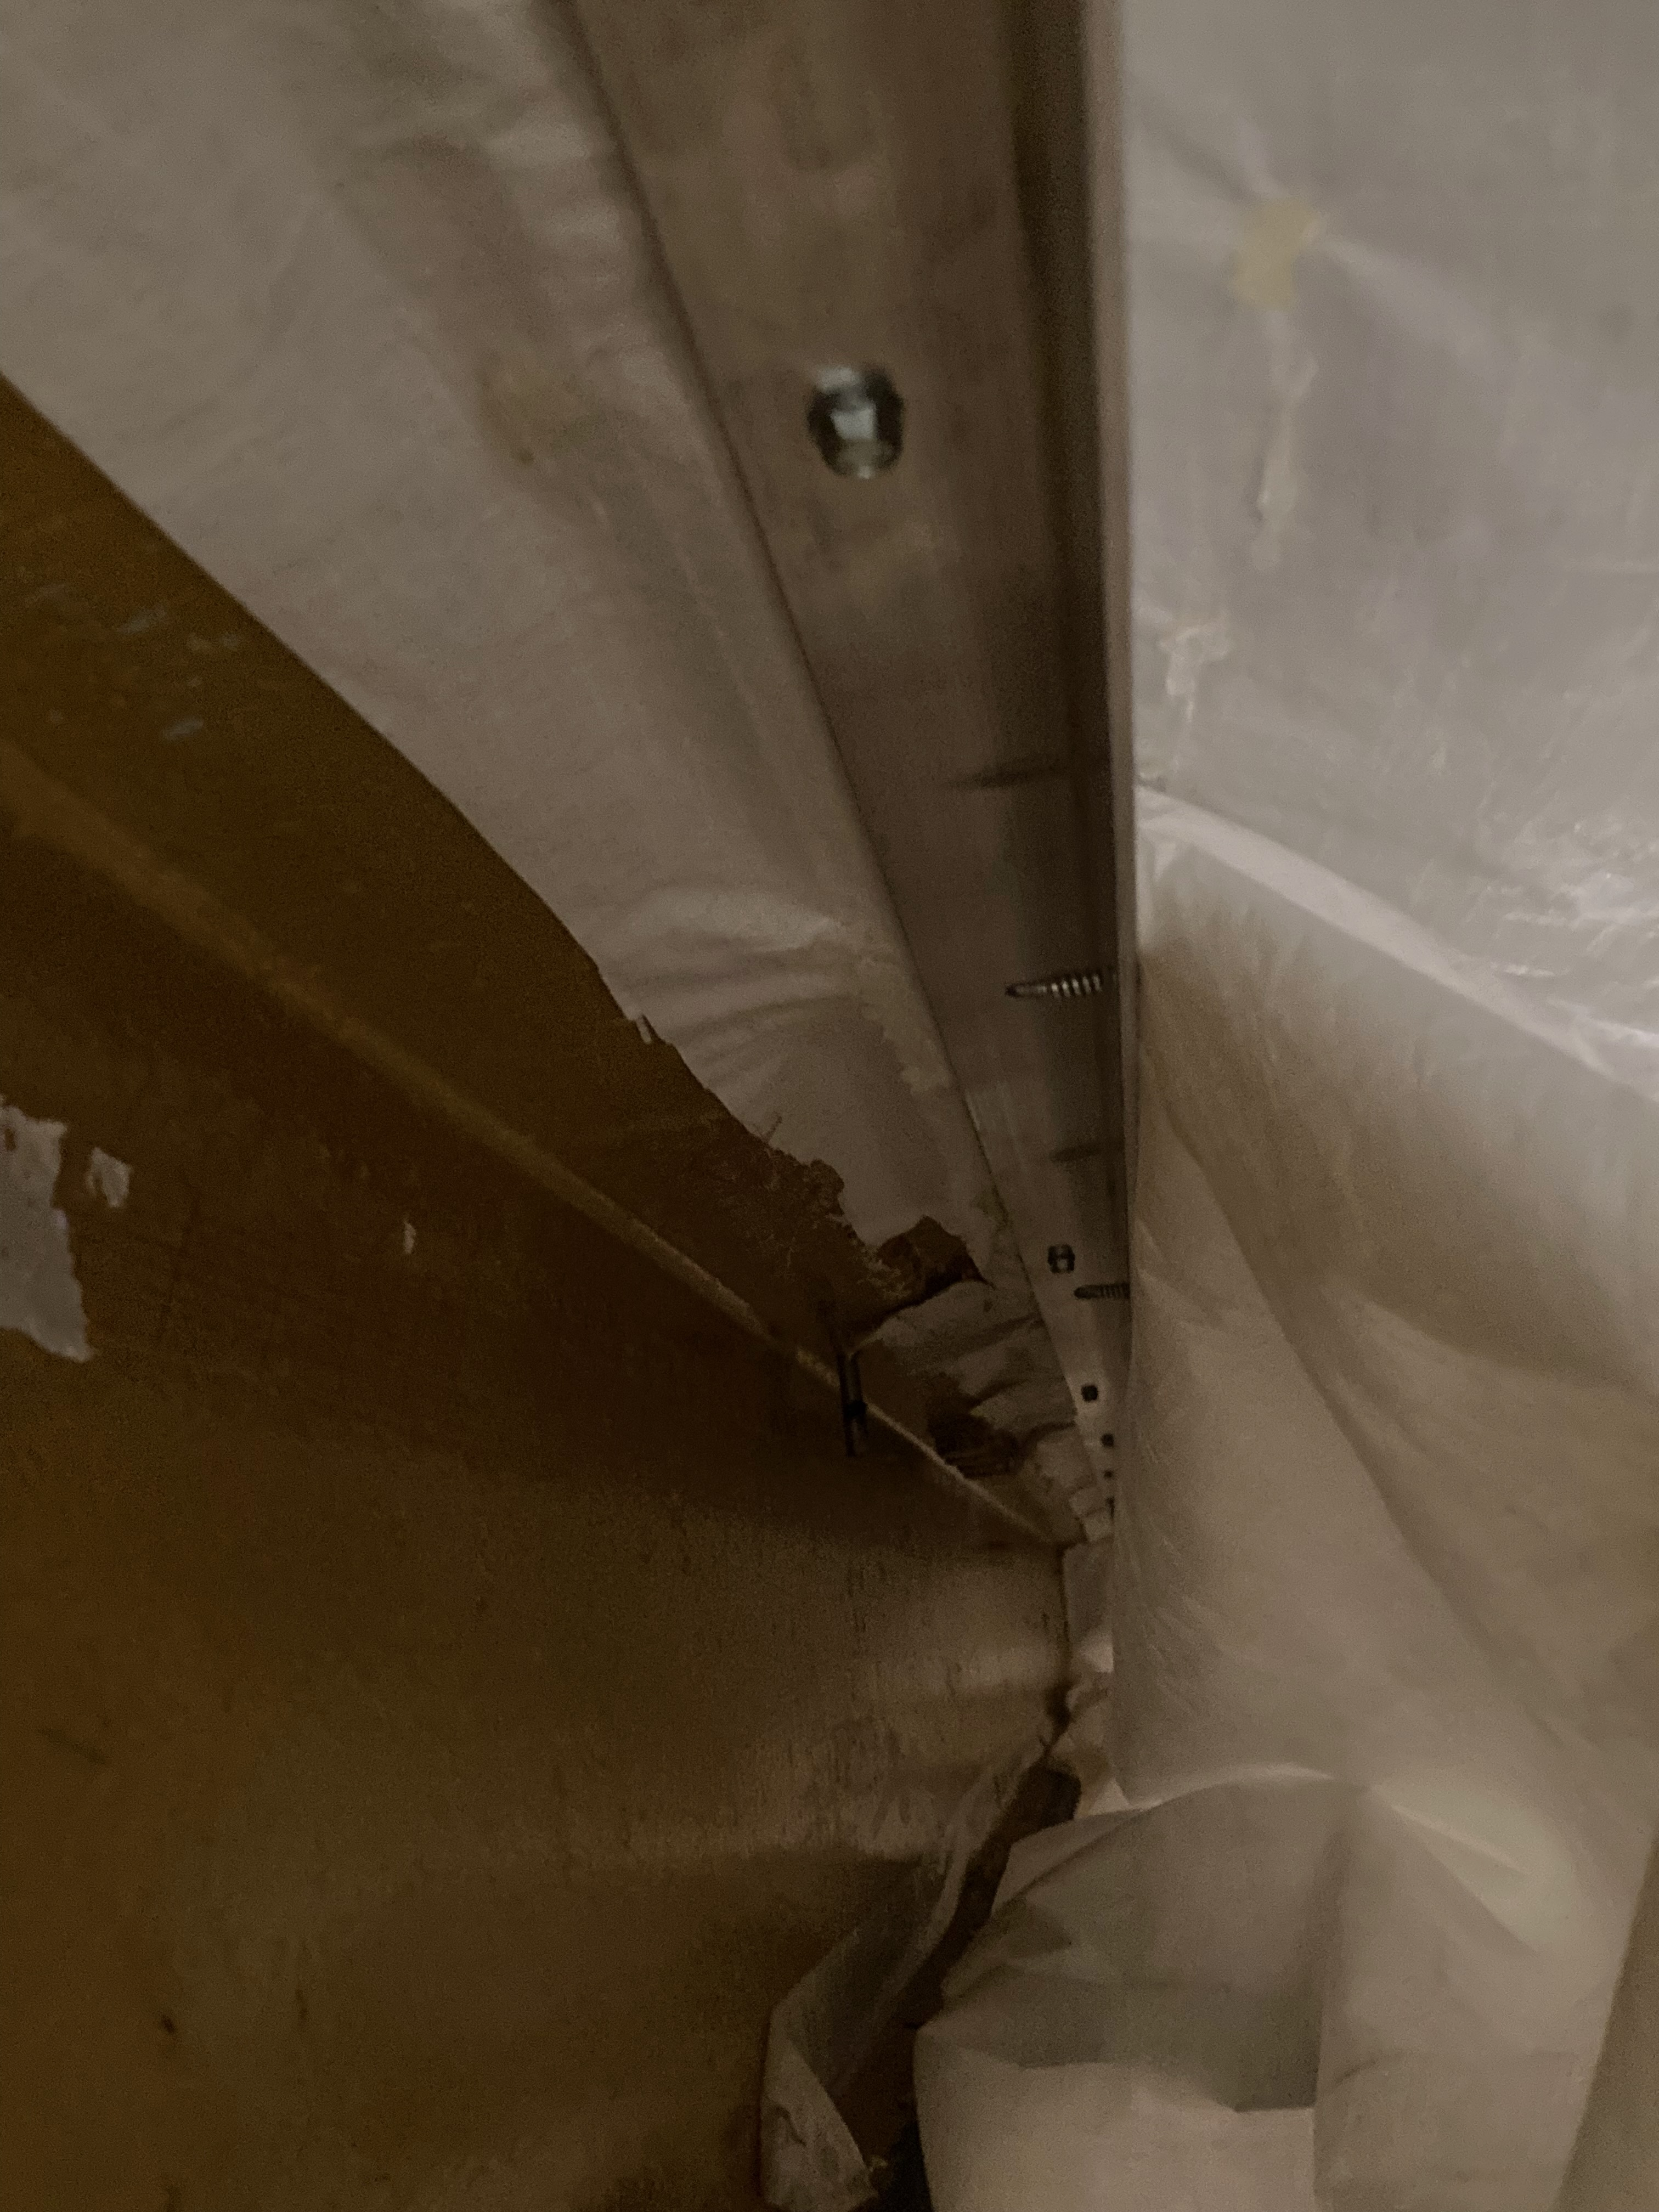
\includegraphics[width=\textwidth]{IMG_5306.jpeg}
	\caption{The DCR I-beam inside the bag}
	\label{fig:inbag}
	\end{subfigure}
	
%	\begin{subfigure}{0.45\textwidth}
%	\includegraphics[width=\textwidth]{CoveredIbeamSouth}
%	\caption{View of the South face of the covered I-beam}
%	\label{fig:cvIbeamS}
%	\end{subfigure}
\end{center}
\end{figure}



\begin{figure}[htbp]
\begin{center}
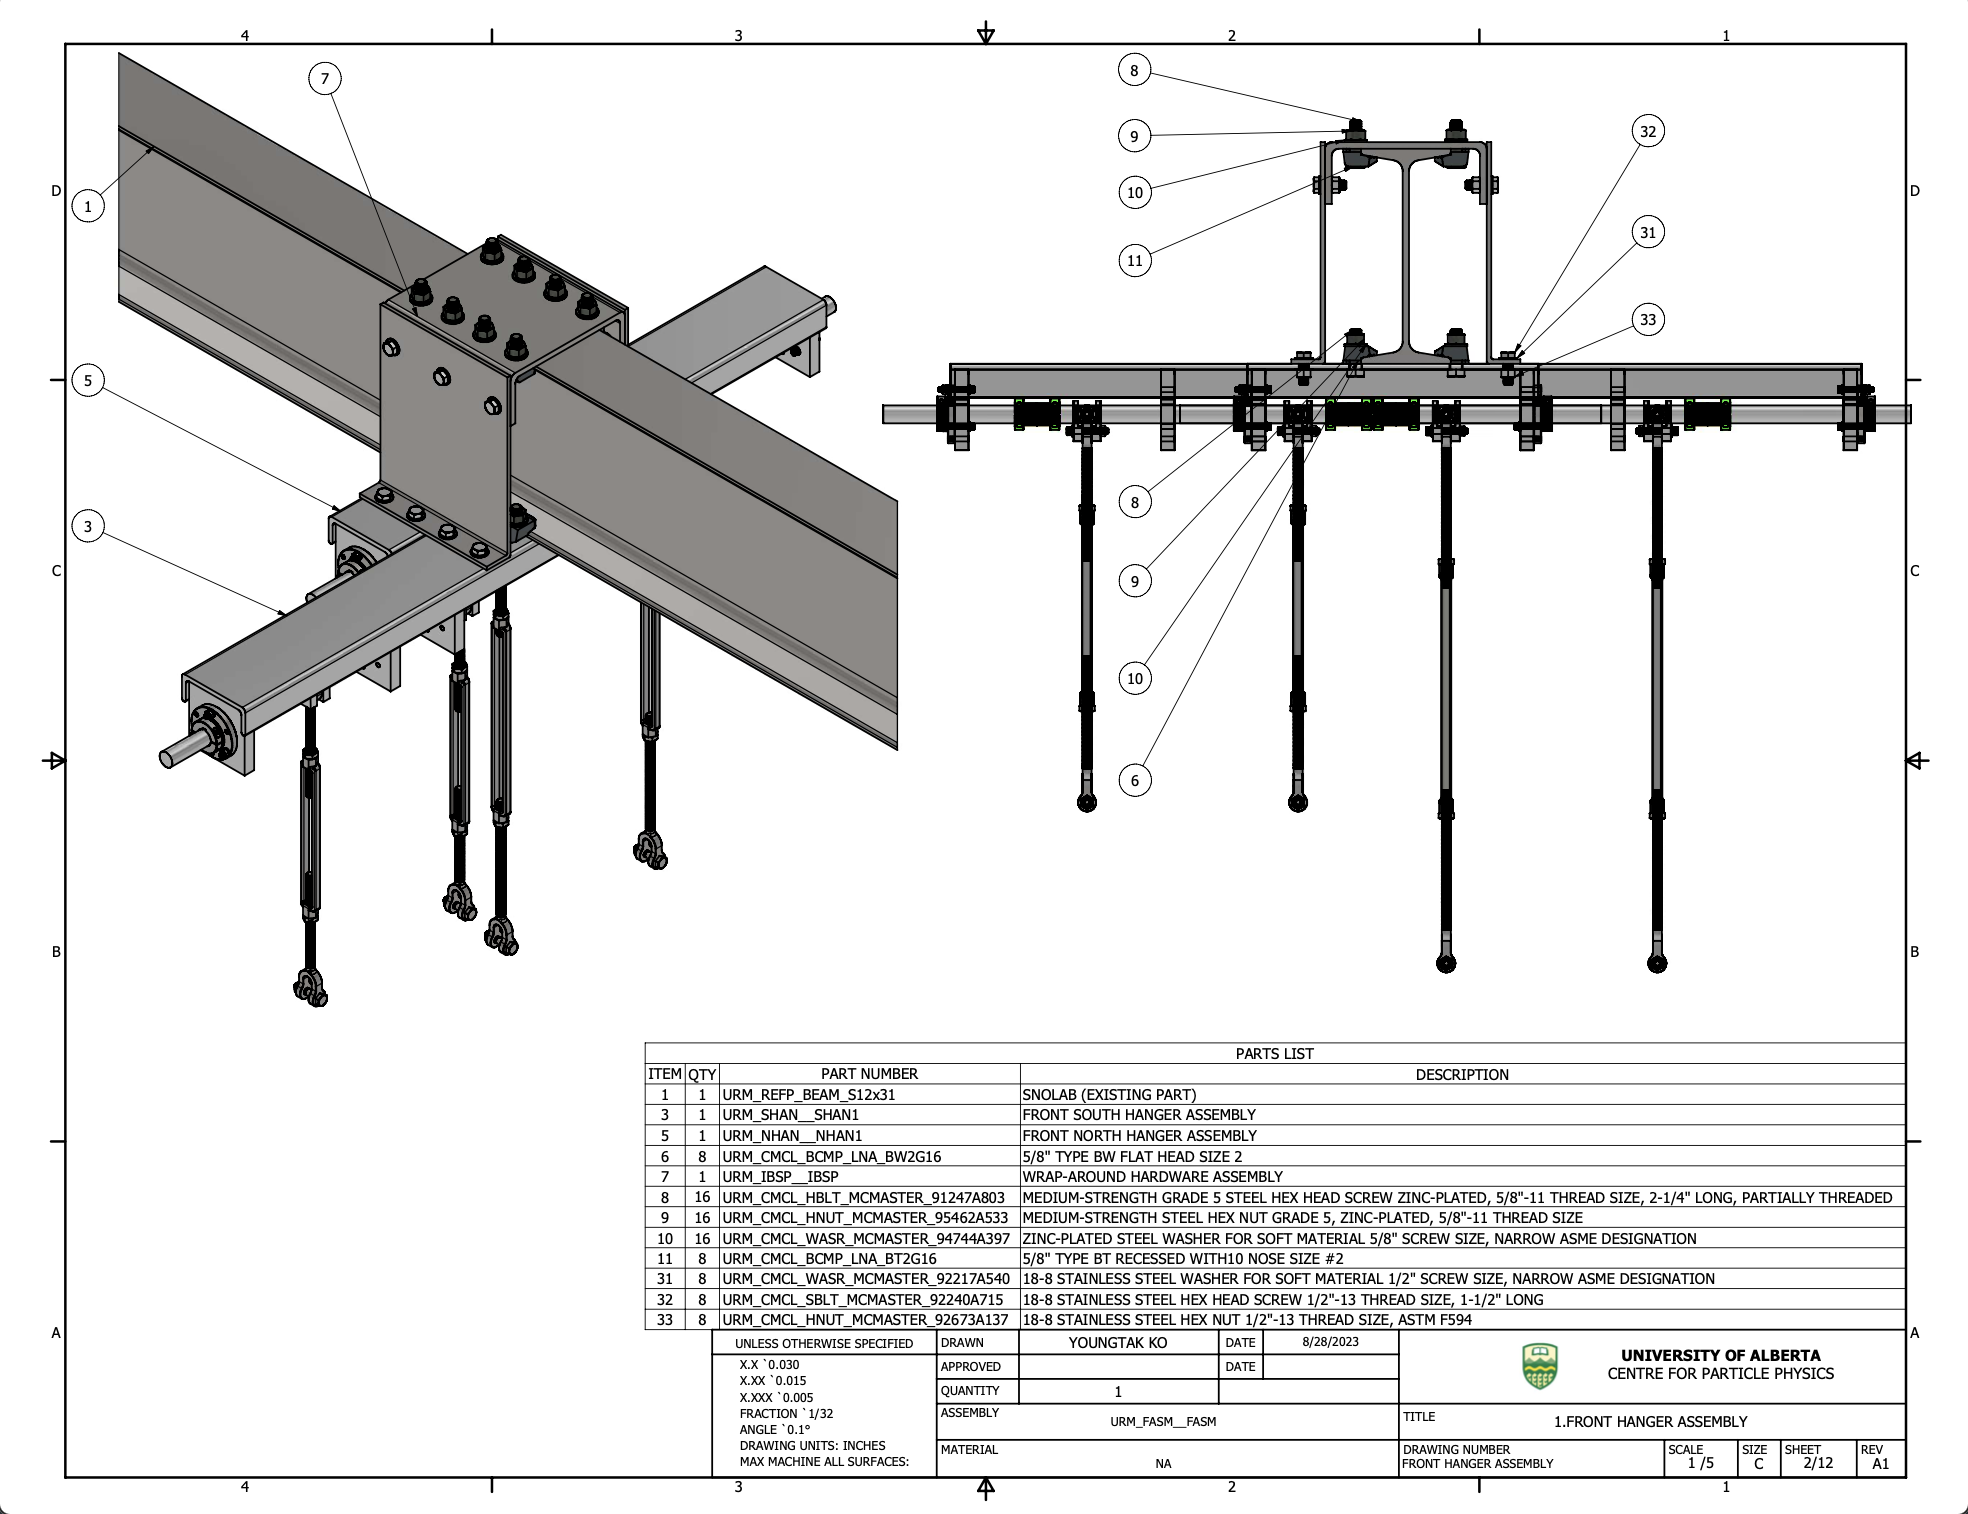
\includegraphics[width=\textwidth]{FrontHangerAssembly.png}
\caption{Front hanger assembly showing the wrap around I-beam clamp}
\label{fig:FHAClamp}
\end{center}
\end{figure}


\subsection{Risks and Mitigation}
To install the wrap around hanger, the workers will be operating at a height at least 60 inches or 170 cm above the deck over the UI. Given that the UI has sensitive equipment on it, using the UI as a platform is not ideal, and ignoring that, the UI is an unstable surface without a rail. Therefore it is assumed that all of the following work will be done using a scaffolding over the UI with a rail in place that can prevent harm to workers or equipment due to potential falls. The scaffold should straddle the UI along the East-West axis to provide access to the length of the I-beam over the UI.  To make the work more ergonomic the scaffolding should be placed so that workers can reach over the DCR ceiling comfortably. This forces a condition where the workers will be working from their knees most of the time; kneepads will be required for the workers. 

\section{Procedure}

\subsection{Pre-Installation Procedures}
\begin{enumerate}
\item Pre-assemble the front hanger off of the I-beam (in the DCR or clean lab) to familiarize all workers with the assembly of the device prior to assembly on the I-beam. Check that all parts will work as intended. 
\item Position drop cloth over UI.
\item Install scaffolding over UI. Vacuum the area around the scaffolding after installation
\item Remove hardware from old lifting mechanism (exception: it may be of value to leave the old front cross-brace to support the side plates during installation instead of installing the new horizontal strut temporarily before moving it to install the bag.)
\item Install dust tent around the scaffolding and secure it to the edge of the UI drop cloth (with clothes pins).
\end{enumerate}

\subsection{Front Hanger Installation Procedure}
\begin{enumerate}
\item Remove strapping securing the I-beam bag from the L brackets on either side of the I-beam. The beam must be exposed to the planned installation position.
\item Peal the DCR tent tarp off both sides of the I-beam in the hanger location. 
\item Cut away a 9" section of the L-bracket from the proposed location of the hanger on both sides of the I-beam. Loosen the screws between the L-bracket and the strapping on the outside of the tent on either side of the work area without completely removing the screws. If adequate shears to cut into the 1/8" aluminum can be identified this can be done in situ; otherwise the whole L-bracket will need to be removed from the DCR and the L-bracket will be cut into the appropriate lengths in the utility drift using a hacksaw with appropriate clean room precautions.
\item Cut  9" wide panels into the tarp to gain access to the top of the I-beam from the tent on both sides of the I-beam. Do not remove the panels from the rest of the tent material. 
\item Cut a matching section from the strapping over the top of the I-beam. If the screws between the angle bracket and the upper strapping has been loosened tighten it again. 
\item Place the upper plate of the hanger over the I-beam. Ideally this should be done from below by sliding the c-section over the I-beam. Clamp the plate to the top flange of the I-beam using the six beam clamps. Allow the free panel of tarp to hang outside of the plate.
\item Secure a piece of tarp 40" in length and 11" in width to the I-beam with double sided tape with enough slack on either side to fold around the downward flange of the top plate of the hanger. Temporarily secure the ends of the tarp with clothes pins. The edges of the tarp should be glued together to make a pocket around the plate. 
\item Lift one of the side plates and align the bolt holes between the top plate and the side plate with the loose end remaining from the ceiling tarp between plates with the free tarp. Puncture all three layers of tarp at each of the three bolt points with an awl or similar tool to ensure alignment. Repeat with the second side plate.
\item Patch the remaining gaps in the tarp with what slack remains from the patch tarp using hot glue. 
\item Disconnect the horizontal arms of the hangers from the vertical plates and I-beam.  
\item Replace the bag along the I-beam by replacing the strapping along the L-bracket. At the front hanger, simply bend the strapping around the plate as necessary.
\item Reconnect the horizontal arms of the hanger with the vertical hanger plates below the bag. Holes will have to be pushed through the bag to accommodate the bolts. Clamp the horizontal arm to the bottom flange of the I-beam using the beam clamps through the I-beam bag.
\item Install the rear hanger by clamping hanger to the lower flange of the I-beam through the bag. 
\item Install the winch using at the former lifting mechanism 
\end{enumerate}

\subsection{Post Installation Procedures}
\begin{enumerate}
\item Clean the interior of the dust tent. Vacuum the surfaces of the scaffolding, and wipe the walls of the dust tent. 
\item Remove the dust tent from the work area.
\item Install hardware on the hanger including straps and turnbuckle.
\item Disassemble the scaffold
\item Remove the UI drop cloth
\item Clean the DCR, starting with the walls and working toward the UI; outer surfaces, vacuum floors, and UI.
\item Repeat cleaning the DCR.
\end{enumerate}

\section{Afterward}

Once this procedure is completed, in situ testing must be completed. The operation of the winches should be tested with the rails alone before any further tests. Alterations must be made to the rails including the front plate and the mounting points at the rear of the rails prior to use with lifting mechanism.  Further testing with the URM will require the parallel completion of the URM scissor table as well as the installation of the URM wheel mounts. Any URM commissioning activities should be completed either before this procedure is complete, or sufficiently isolated in time that the DCR is returned to a clean room status with fewer than 200 counts of 0.5 $\mu$m particulates per $m^{3}$. Presumably this includes multiple complete cleanings of the DCR.

\end{document}